\documentclass[11pt,letterpaper]{article}
\usepackage[margin=0.85in]{geometry}
\usepackage{amsmath,amssymb,mathtools,graphicx,booktabs,array,microtype,xcolor,hyperref,fancyhdr}
\hypersetup{colorlinks=true,linkcolor=blue!45!black,urlcolor=blue!50!black}
\newcommand{\Z}{\mathbb Z}\newcommand{\R}{\mathbb R}\newcommand{\dd}{\mathrm d}\newcommand{\F}{\mathcal F}
\pagestyle{fancy}\fancyhf{}\lhead{Physics of Tabla}\rhead{Mathematics of Rhythm}\cfoot{\thepage}
\title{\textbf{The Mathematics of Musical Rhythm}\\[5pt]\large Dirac Combs, Fourier Analysis, Cyclic Groups, and Taal}
\author{An educational companion to \emph{The Physics of Tabla Vibration and Musical Harmony}}
\date{November 2026}
\begin{document}\maketitle
\begin{abstract}
This standalone tutorial develops a mathematical description of rhythm with examples drawn especially from Hindustani taal. Ideal rhythmic events are modeled with Dirac impulses; their periodicity is studied using Fourier transforms, discrete Fourier series, cyclic groups, and phase variables. We examine teentaal and jhaptal, derive modular conditions for a tihai to resolve on sam, and connect stroke timing to the sound of a physical tabla membrane. The figures are reproducible from the included Python script. Illustrative accent weights are explicitly distinguished from ethnographic claims or measured performances.
\end{abstract}
\tableofcontents
\section{Musical scope and a necessary qualification}
Western rhythms are not universally linear and Indian rhythms are not exclusively cyclical. Western meters and ostinatos are often periodic, while Hindustani performances have developmental, nonperiodic, and expressive aspects. The mathematically fruitful distinction is not the existence of a cycle but the \emph{functional prominence} of an identified return to \emph{sam} and of subdivisions marked by \emph{tali}, \emph{khali}, and \emph{vibhag}. Musical meanings exceed any impulse-train model; foundational discussion is given by Clayton~\cite{clayton} and the rhythm-geometry perspective by Toussaint~\cite{toussaint}.

\section{From isolated strokes to the Dirac comb}
A point event at time $t_j$ can be represented in the sense of distributions by $\delta(t-t_j)$. A sequence of unit strokes separated by time $T$ is
\begin{equation}\operatorname{III}_T(t)=\sum_{n\in\Z}\delta(t-nT).\label{eq:comb}\end{equation}
The delta is an idealized event marker, \emph{not} a physically emitted sound pressure waveform. Under the Fourier convention
\begin{equation}\tilde x(f)=\int_{-\infty}^{\infty}x(t)e^{-2\pi i f t}\,\dd t,\end{equation}
Poisson summation gives the distributional identity
\begin{equation}\boxed{\F\{\operatorname{III}_T\}(f)=\frac1T\sum_{k\in\Z}\delta\!\left(f-\frac{k}{T}\right).}\label{eq:poisson}\end{equation}
Thus equally spaced events in time give spectral lines spaced by $1/T$. Finite performances instead exhibit broadened peaks due to finite observation windows and timing variability. A real bol has a waveform $h(t)$; for identical strokes the output is $s=h*\operatorname{III}_T$ and $\tilde s=\tilde h\,\widetilde{\operatorname{III}}_T$. The attack, ringing, and damping of $h$ belong to the membrane-acoustics companion manuscript.

\section{Weighted cycles: teentaal and jhaptal}
For a cycle containing $N$ matras, define a $T$-spaced pattern $p(t)=\sum_{j=0}^{N-1}a_j\delta(t-jT)$ and repeat it indefinitely:
\begin{equation}x(t)=\sum_{n\in\Z}\sum_{j=0}^{N-1}a_j\delta(t-(nN+j)T).\label{eq:cycle}\end{equation}
The coefficients $a_j$ can encode measured loudness, a selected bass-band amplitude, an abstract accent, or one channel of a multicomponent stroke description. They are \emph{not} universally prescribed for a taal. In teentaal, $N=16$ and its four vibhags have lengths $4+4+4+4$; their boundary matras are $1$ (sam), $5$ (tali), $9$ (khali), and $13$ (tali). Jhaptal has $N=10$ and groups $2+3+2+3$, with the boundary markers at matras $1,3,6,8$ (sam, tali, khali, tali respectively). \emph{Khali does not mean silence}: its sound may emphasize a different balance of bass and treble strokes.
\begin{figure}[ht]\centering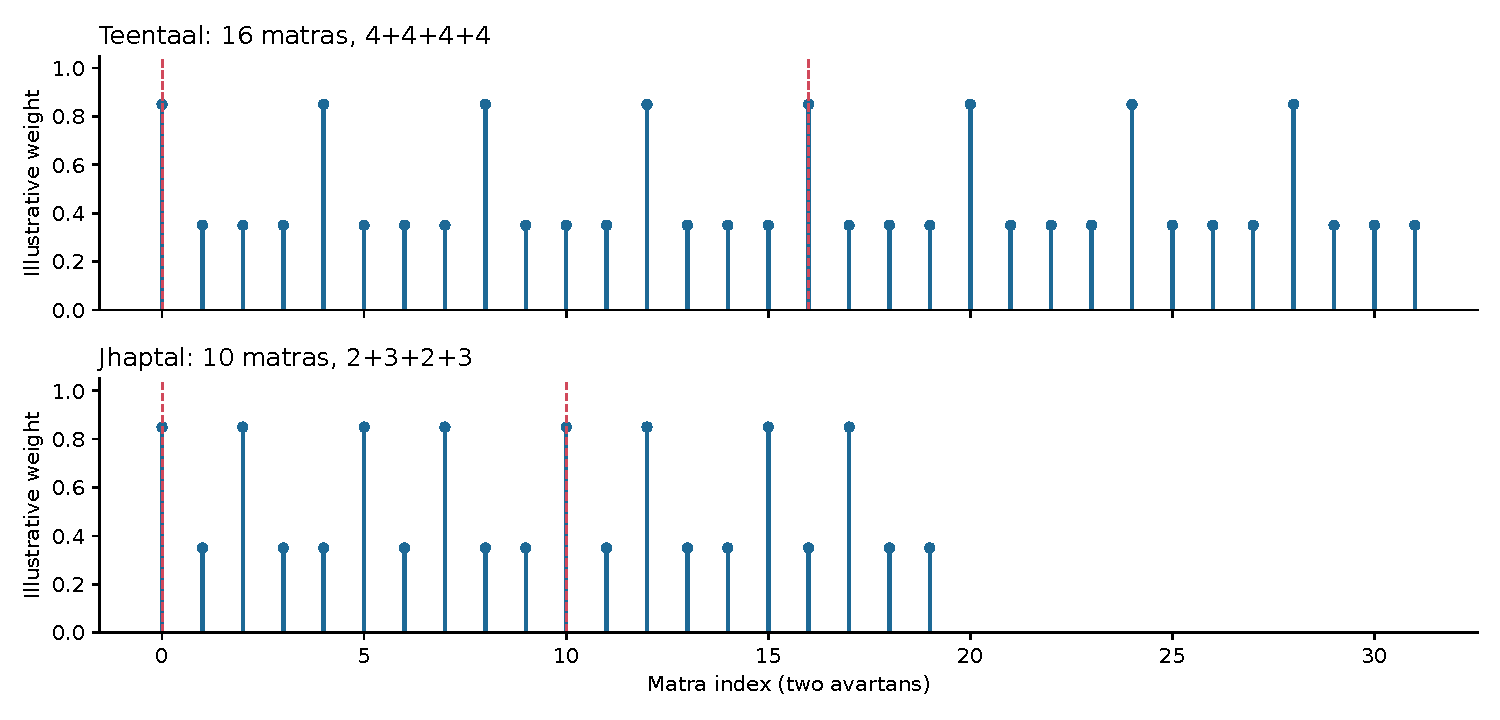
\includegraphics[width=.96\linewidth]{figures/impulse_trains.pdf}\caption{Two idealized periodic event trains. Marker heights are illustrative grouping weights, not measured dynamics or a complete transcription of either theka. Dotted lines mark cycle boundaries.}\end{figure}
\begin{figure}[ht]\centering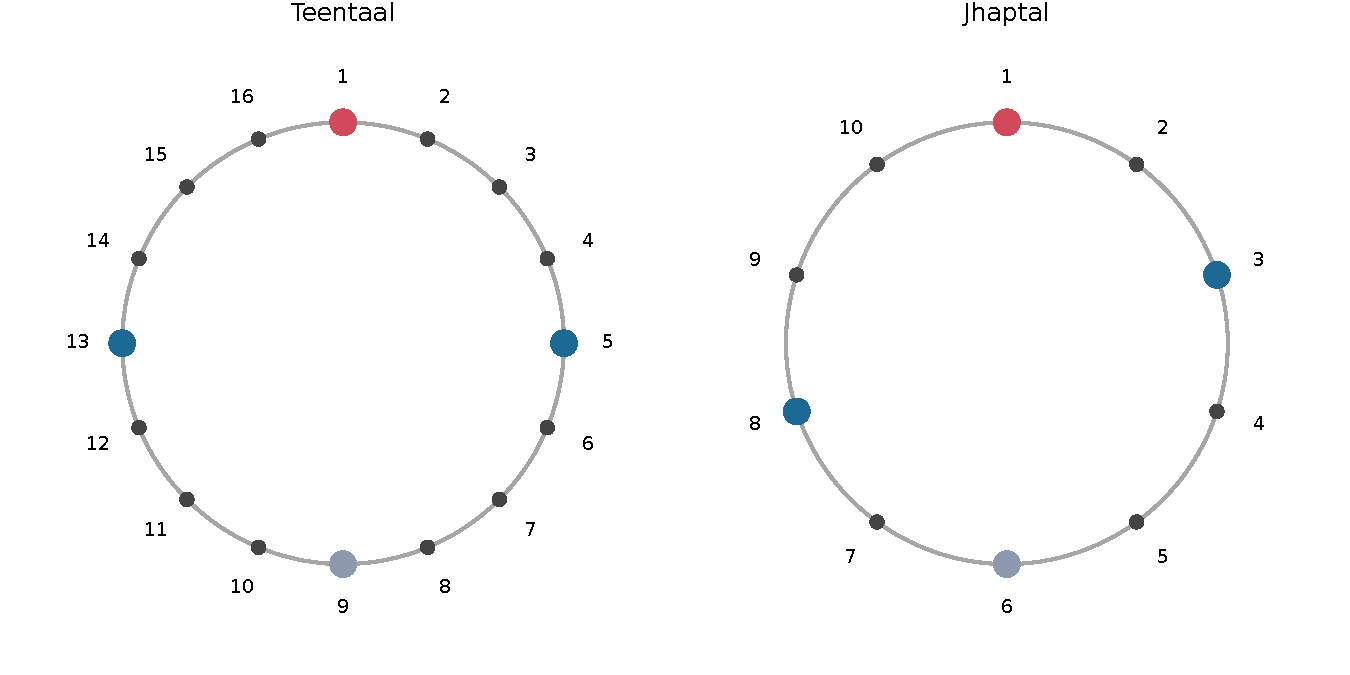
\includegraphics[width=.86\linewidth]{figures/cycle_diagrams.pdf}\caption{Matras placed around an oriented circle; red denotes sam, blue denotes other tali boundaries, gray denotes khali. The angular position is an explanatory representation, not an acoustic measurement.}\end{figure}

\section{Fourier transform of a weighted cycle}
Write the single-cycle Fourier transform as $\tilde p(f)=\sum_{j=0}^{N-1}a_je^{-2\pi ifjT}$. The full signal is $x=p*\operatorname{III}_{NT}$, so
\begin{align}
\tilde x(f)&=\frac{1}{NT}\sum_{k\in\Z}P_k\,\delta\!\left(f-\frac{k}{NT}\right),\\
P_k&=\sum_{j=0}^{N-1}a_je^{-2\pi ikj/N}.\label{eq:dft}
\end{align}
The $P_k$ are the length-$N$ discrete Fourier transform (DFT) of the within-cycle weights. This gives an interpretation: the full-cycle duration controls spectral line locations, while the pattern within a cycle controls their complex amplitudes. Real-valued data satisfy $P_{N-k}=P_k^*$ and $P_{k+N}=P_k$. If all weights are equal, only frequencies corresponding to the underlying matra-rate comb remain, even if an analyst imposes an artificial $N$-beat grouping: \emph{sound alone need not disclose perceived metrical structure}.

\section{Phase, sam, and rhythm on a circle}
Physical time lies on $\R$, while normalized position in an ideal constant-tempo avartan is
\begin{equation}\boxed{\theta(t)=\frac{2\pi t}{NT}\pmod{2\pi}.}\label{eq:phase}\end{equation}
The cycle lives on the unit circle $S^1$ and sam is conventionally $\theta=0$. Each matra of teentaal advances phase by $2\pi/16=\pi/8$. A performed phrase may have many events and subdivisions without altering the basic metrical phase. With expressive tempo, replace Eq.~\eqref{eq:phase} by $\theta(t)=\int_0^t\Omega(u)\dd u\pmod{2\pi}$, where $\Omega$ is a time-varying cycle angular speed. This is a model of phase tracking, not a claim that a human performer maintains a mathematically exact oscillator.

\section{Cyclic groups, shifts, and missing phase information}
Assign the matras to the cyclic group $\Z_N$. A shift by $\ell$ acts as $(\mathcal T_\ell a)_j=a_{j-\ell\pmod N}$. Applying the DFT definition yields
\begin{equation}\boxed{\widehat{\mathcal T_\ell a}(k)=e^{-2\pi ik\ell/N}\widehat a(k).}\end{equation}
Therefore $|\widehat{\mathcal T_\ell a}(k)|=|\widehat a(k)|$. Two different alignments relative to sam can have indistinguishable DFT magnitude spectra but different complex phases. Spectral power cannot by itself identify whether a motif begins on sam or khali. This is a meaningful limit of magnitude-only analysis, rather than a failure of the Fourier transform.
\begin{figure}[ht]\centering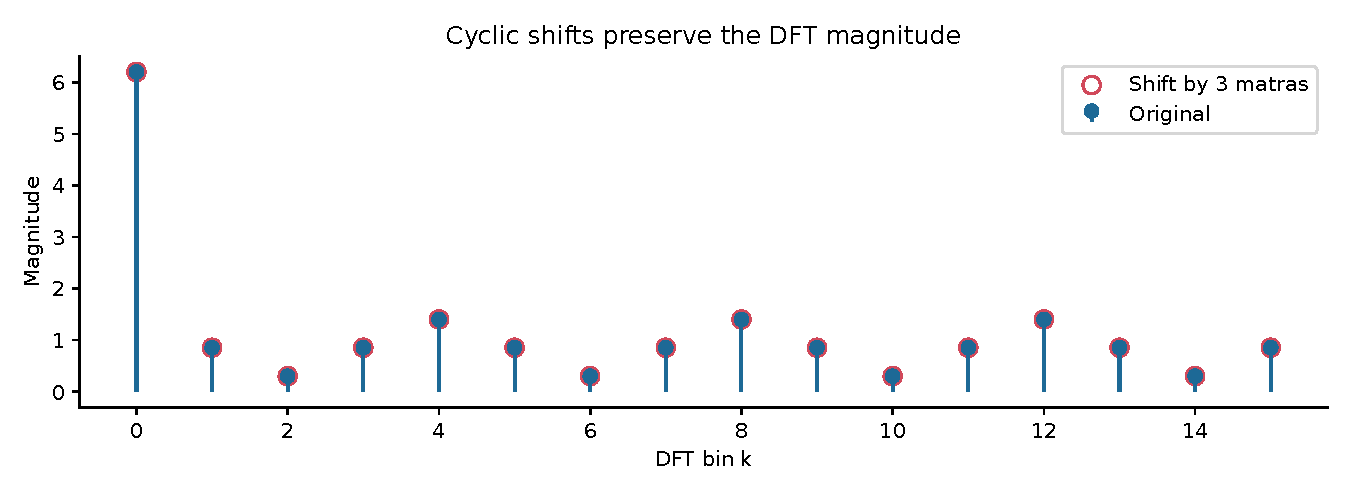
\includegraphics[width=.88\linewidth]{figures/dft_shift.pdf}\caption{Magnitude DFT of an illustrative 16-event weight vector and the same vector shifted by three positions. The plotted spectra coincide; their complex Fourier phases do not.}\end{figure}

\section{Tihai as modular phase matching}
Model a tihai as three repetitions of the same motif. Define $L$ to mean the \emph{elapsed duration} from the start of one phrase to its terminal stroke, in matra units; let $g$ be any additional gap after the terminal stroke before the next phrase starts. The three starting positions are $n_0$, $n_0+(L+g)$, and $n_0+2(L+g)$. The last stroke lands at $n_f=n_0+3L+2g$. For an $N$-matra taal, the resolution-to-sam condition is
\begin{equation}\boxed{n_0+3L+2g\equiv0\pmod N.}\label{eq:tihai}\end{equation}
Example: in teentaal let $N=16$, $L=4$, $g=0$. Then $n_0\equiv4\pmod{16}$, meaning the first phrase starts at matra 5 and the terminal stroke of the third phrase lands on the next sam (elapsed index 16). The phrases can contain arbitrary internal strokes consistent with their defined terminal duration. Other counting conventions (e.g., length as the number of occupied grid cells) must modify the equation accordingly.
\begin{figure}[ht]\centering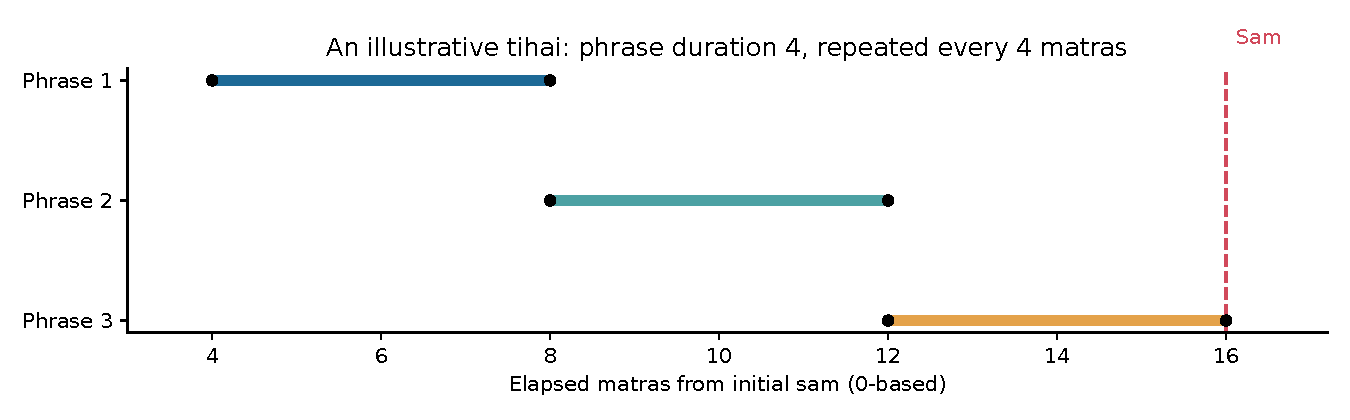
\includegraphics[width=.93\linewidth]{figures/tihai.pdf}\caption{An illustrative three-phrase schedule. The red dashed line represents the next sam. The horizontal spans indicate phrase durations, not continuous notes.}\end{figure}

\section{Layakari, subdivision and polyrhythm}
A subdivision $m$ times faster than the base matra uses event spacing $T/m$; a superposed sequence at another rate produces overlapping modular structures. For rational frequency ratios $p:q$, their grids share a common phase after integer subdivisions, and one can study coincidence using least common multiples. In a $3$-against-$4$ pattern over one common duration $D$, three equal pulses occur at $jD/3$ and four at $jD/4$. Their only simultaneous onsets in the half-open interval $[0,D)$ occur at zero; both align again at $D$. These ideal patterns provide a starting point, but actual layakari includes idiom, articulation, accent and compositional context that simple pulse ratios do not capture.
\begin{figure}[ht]\centering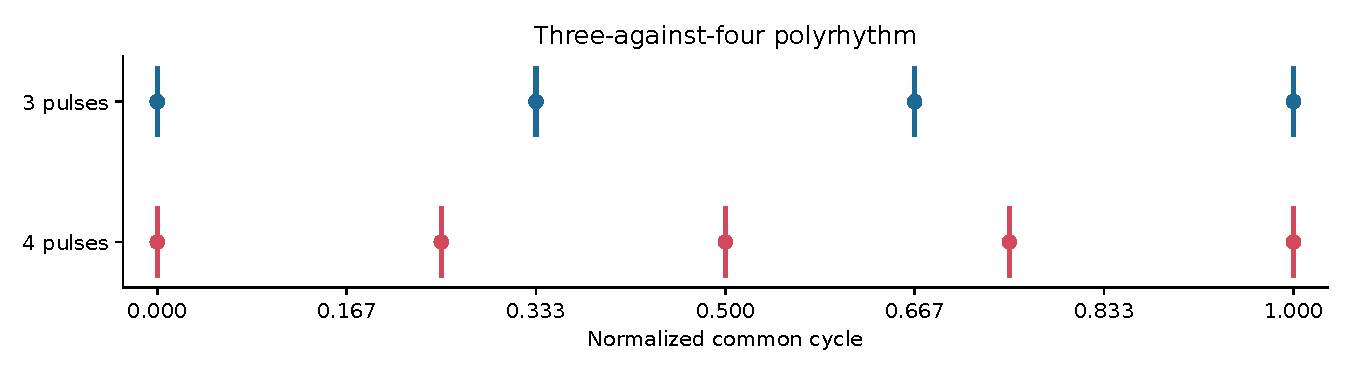
\includegraphics[width=.9\linewidth]{figures/polyrhythm.pdf}\caption{Idealized three-against-four subdivision over a common duration. Coincident endpoints indicate alignment at the cycle boundary.}\end{figure}

\section{Relating timing to the acoustics of an actual tabla}
For more realistic sound, label each event by a bol $b_j$ and use its own impulse response $h_{b_j}$:
\begin{equation}\boxed{s(t)=\sum_j A_jh_{b_j}(t-t_j).}\label{eq:audio}\end{equation}
This is a \emph{sum of shifted stroke responses}, and only reduces to the convolution of a single fixed waveform with an event train when all $h_{b_j}$ are the same. Finger damping, contact location, excitation of membrane normal modes, and bayan/dayan selection alter $h_b$. The timing representation describes \emph{when}; the membrane response describes \emph{what sounds}. Stroke-to-stroke variations and nonlinear contact effects limit the adequacy of a fixed waveform library.

\section{Cross-cultural interpretation without false dichotomies}
Western metrical systems use beats, measures, accents, downbeats, and many cycles; Hindustani taal uses matras, avartans, vibhags, tali, khali, and a particularly salient return to sam. A comparison should investigate the performance roles of these concepts rather than declaring that Western musical time is a line and Indian musical time a circle. Any abstract $\Z_N$ model must additionally represent tempo changes, phrase boundaries, microtiming, timbre, and musicians' expectations to describe actual performance. Clayton~\cite{clayton} studies rhythmic organization in cross-cultural perspective; CompMusic provides annotated materials and corpus analyses for computational tests~\cite{compmusic,corpus}.

\section{Suggested computational and empirical experiments}
\begin{enumerate}
\item Record and annotate two or more avartans of a traditional theka, including stroke labels and onset times; compare with the ideal grids shown here.
\item Compute complex DFT coefficients of selected measurable features (onset strength, spectral centroid, bass energy), report magnitude \emph{and} phase, and investigate their behavior under cyclic shifts.
\item Compare teentaal and jhaptal after normalizing total duration, and separately compare different $N$ without normalization to distinguish grouping from periodicity.
\item Generate tihais by solving Eq.~\eqref{eq:tihai} for specified phrase length, gaps and desired ending cycle; check the terminal-stroke convention explicitly.
\item Construct an audio synthesizer from recorded bol waveforms using Eq.~\eqref{eq:audio} and investigate finger damping and resonance as discussed in the companion acoustics tutorial.
\item Study phase tracking under variable tempo and imperfect timing using annotated datasets rather than assuming an exact Dirac comb.
\end{enumerate}

\section*{Reproducibility and limitations}
Run \texttt{python scripts/generate\_figures.py} from this directory (requires NumPy and Matplotlib). All five included figures are synthetic pedagogical diagrams. No measured tabla audio or fitted timing data were used. The plotted weights are chosen to explain mathematical structure, not to prescribe authentic accent patterns for a tradition. This manuscript and the companion membrane-acoustics manuscript are intended as separate documents within the same public project.

\begin{thebibliography}{9}
\bibitem{clayton} M. Clayton, \emph{Time in Indian Music: Rhythm, Metre, and Form in North Indian R\=ag Performance}, Oxford University Press (2000). \url{https://academic.oup.com/book/49788}.
\bibitem{toussaint} G. T. Toussaint, \emph{The Geometry of Musical Rhythm: What Makes a ``Good'' Rhythm Good?}, CRC Press (2013). \url{https://books.google.com/books?id=ZlKfh83AJEEC}.
\bibitem{compmusic} CompMusic, \emph{Hindustani Music Rhythm Dataset}. \url{https://compmusic.upf.edu/ta/hindustani-rhythm-dataset}. Also see \url{https://zenodo.org/records/1264742}.
\bibitem{corpus} CompMusic, \emph{Aspects of Tempo and Rhythmic Elaboration in Hindustani Music: A Corpus Study}, \emph{Frontiers in Digital Humanities} (2017), DOI: \href{https://doi.org/10.3389/fdigh.2017.00020}{10.3389/fdigh.2017.00020}.
\bibitem{tabla} CompMusic, \emph{Tabla Solo Dataset}. \url{https://compmusic.upf.edu/te/tabla-solo-dataset}.
\bibitem{fourier} J. K. Hunter, \emph{Distributions and the Fourier Transform}, lecture notes, \url{https://www.math.ucdavis.edu/~hunter/book/ch11.pdf}, sections on the Dirac comb and Poisson summation.
\end{thebibliography}
\end{document}
